\documentclass[acmsmall,review,nonacm]{acmart}\settopmatter{printfolios=true,printccs=false,printacmref=false}

\AtBeginDocument{%
	\providecommand\BibTeX{{%
			\normalfont B\kern-0.5em{\scshape i\kern-0.25em b}\kern-0.8em\TeX}}}

\setcopyright{acmcopyright}
\copyrightyear{2018}
\acmYear{2018}
\acmDOI{10.1145/1122445.1122456}

\usepackage{listings}
\usepackage{lipsum}
\usepackage{xcolor}
\usepackage{multirow}


%% These commands are for a PROCEEDINGS abstract or paper.
\acmConference[Woodstock '18]{Woodstock '18: ACM Symposium on Neural
	Gaze Detection}{June 03--05, 2018}{Woodstock, NY}
\acmBooktitle{Woodstock '18: ACM Symposium on Neural Gaze Detection,
	June 03--05, 2018, Woodstock, NY}
\acmPrice{15.00}
\acmISBN{978-1-4503-XXXX-X/18/06}


\begin{document}
	
	\title{Fine-grained Reductions Around Context-Free Path Querying}
	
	\author{Aleksandra Istomina}
	\email{aleksandra2999@mail.ru}
	\affiliation{%
		\institution{Saint Petersburg State University}
		\city{Saint Petersburg}
		\country{Russia}
	}
	\affiliation{%
	\institution{JetBrains Research}
	\city{Saint Petersburg}
	\country{Russia}
	}

    \author{Research advisor: Semyon Grigorev}
    \affiliation{%
    	\institution{Saint Petersburg State University}
    	\city{Saint Petersburg}
    	\country{Russia}
    }
    \affiliation{%
    	\institution{JetBrains Research}
    	\city{Saint Petersburg}
    	\country{Russia}
    }
	
	\newcommand\todo[1]{{\color{violet}#1}}
	\newcommand\db[1]{{\color{red}#1}}
	\newcommand\question[1]{{\color{cyan}#1}}


	\maketitle
	
	\todo{graduate, ACM number: 4678238}
	
	\section{Introduction}
	
	\subsection{\todo{brief description of the problem, areas of usage, idea of solution}}
	
	cfpq appears in bioinformatics, graph databases, static code analysis
	
	finding valid paths between vertices
	
	\subsection{\todo{problems with current cfpq results}}
	
	several cubic algorithms exist
	
	can we do significantly better? no such algorithm had been found for several decades
	
	maybe we can prove that no such algorithm exist under some hypothesis
	
	\subsection{\todo{main problem}}
	
	fine-grained complexity has some results in the area
	
	results are scattered, have no structure
	
	maybe everything is already proven
	
	\subsection{\todo{main goals, overview}}
	
	collect existing results into easy-to-read form
	
	state open problems
	
	\section{Preliminaries}
	
	cfg, directed graph, cfl reachability and recognition, note on Dyck-1, fine-grained reduction
	
	\section{Main Results}
	
	\begin{figure}[!htp]
		
		\begin{center}  
			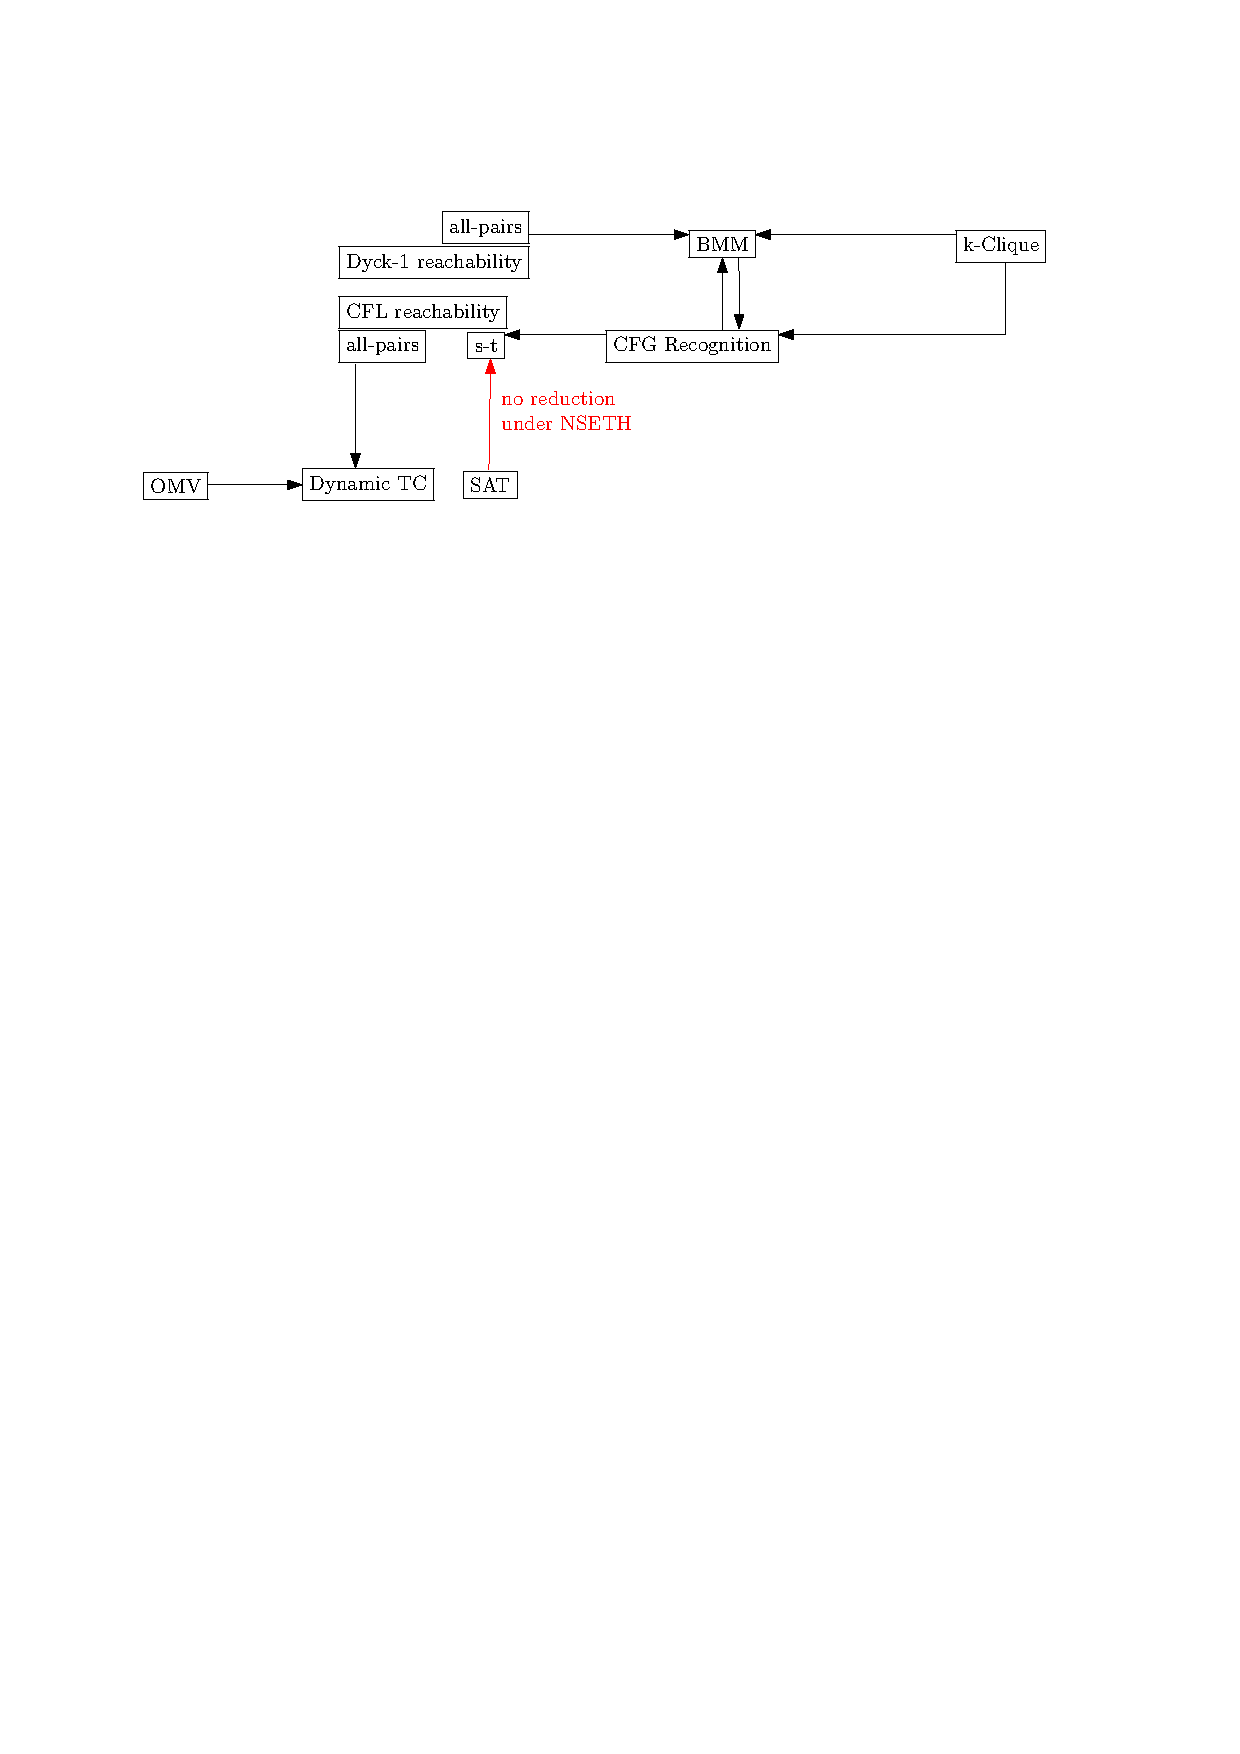
\includegraphics[scale = 0.6]{map_popl.pdf}
		\end{center}
	
		\caption{arrow - reduction the other side. blue arrow - open problem. \\
		\todo{!!!check reduction OV to Dyck-1}}
		
	\end{figure}
	
	In \cite{valiant1975general}
	
	\subsection{\todo{existing problems and hypotheses}}
	
	shortly describe problems (OV, BMM, LED, SAT, DTC) on map and hypotheses about them + NSETH
	
	\subsection{\todo{existing reductions}}
	
	dynamic TC to all-pairs
	
	BMM to Dyck-1
	
	s-t -> cfg -> bmm => no combinatorial algorithm
	
	short s-t certificates => no reduction from SAT
	
	\subsection{\todo{OV to Dyck-1}}
	
	$\mathcal{O}(n^{2 - \epsilon}) \Rightarrow \mathcal{O}(n^{2 - \epsilon})$
	
	idea based on reduction APA to Dyck-1 
		
	\subsection{\todo{open problems}}
	
	global: subcubic cfpq
	
	s-t vs all-pairs reachability: comparison with triangles detection problem
	
	\section{Conclusion and Future work}
	
	part of global work to determine existence of subcubic cfpq algorithm
	
	formalisation of naive reduction LED to s-t
	
	possible reduction form APSP and reformulations
	
	\section{Acknowledgments}
	
	\bibliographystyle{ACM-Reference-Format}
	\bibliography{map}
	
	\appendix
	
\end{document}
\endinput
